\section{Introduction}\label{introduction-002}

This auxiliary tool generates HVAC performance curves in EnergyPlus curve object format. For each set of performance data entered, Capacity and EIR performance curves are generated, and these curves are generated either as a function of temperature(s) or flow fraction. The Capacity and EIR of Cooling DX Coils as a function of temperatures require only Biquadratic curve whereas Capacity and EIR of Heating DX Coils may use Biquadratic, Cubic and Quadratic curves. The selection of either of these curves is dependent on availability of performance data. The Capacity and EIR as a function of flow fraction allows either Cubic or Quadratic curve type. The curve types allowed are:

Biquadratic: \(\text{CurveValue} = a_0 + a_1 X + a_2 X^2 + a_3 Y + a_4 Y^2 + a_5 XY\)

Cubic: \(\text{CurveValue} = a_0 + a_1 X + a_2 X^2 + a_3 X^3\)

Quadratic: \(\text{CurveValue} = a_0 + a_1 X + a_2 X^2\)

These performance curves as a function of temperatures are generated for a given set of input data at a given speed. The curves as a function of flow fraction are generated at the rated temperature conditions. The rated test condition is the AHRI standard test condition (AHRI 2003;2007; 2008). The AHRI standard test condition may vary by the equipment type. For multiple speeds or multiple stage DX Coils, different curve sets can be generated by entering a different set of data for each speed or stage at a time. The tool automatically populates the labels for each data inputs variable when users select the Coil Type, Independent Variables, Curve Type, and Units. The curve fit tool interface in Figure~\ref{fig:main-menu-screen-of-the-weather-converter} shows labels selected to generate capacity and EIR biquadratic curves as function of temperatures for DX cooling coil.

\begin{figure}[hbtp] % fig 33
\centering
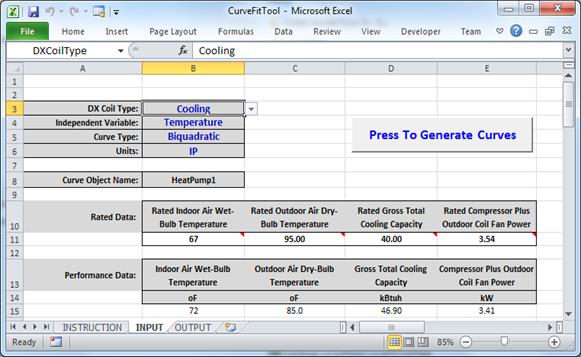
\includegraphics[width=0.9\textwidth, height=0.9\textheight, keepaspectratio=true]{media/image034.jpg}
\caption{Curve Fit Tool Input Interface \protect \label{fig:curve-fit-tool-input-interface}}
\end{figure}

The tool can be used for Coil:Cooling:DX:SingleSpeed, Coil:Heating:DX:SingleSpeed, Coil:Cooling:DX:TwoSpeed (high and low speed) , CoilPerformance:DX:Cooling (each stage), and any HVAC equipment that use Biquadratic, Cubic or Quadratic curves. To add this flexibility generic input data labels can be populated by selecting ``Other'' for DX Coil Type input field, located in Cell B3 in Figure~\ref{fig:curve-fit-tool-input-interface}.
